% last updated in April 2002 by Antje Endemann
% Based on CVPR 07 and LNCS, with modifications by DAF, AZ and elle, 2008 and AA, 2010, and CC, 2011; TT, 2014

\documentclass[runningheads]{llncs}
\usepackage{graphicx}
\usepackage{amsmath,amssymb} % define this before the line numbering.
\usepackage{ruler}
\usepackage{color}
\usepackage[width=122mm,left=12mm,paperwidth=146mm,height=193mm,top=12mm,paperheight=217mm]{geometry}


\newcommand*{\affaddr}[1]{#1} % No op here. Customize it for different styles.
\newcommand*{\affmark}[1][*]{\textsuperscript{#1}}

\begin{document}
% \renewcommand\thelinenumber{\color[rgb]{0.2,0.5,0.8}\normalfont\sffamily\scriptsize\arabic{linenumber}\color[rgb]{0,0,0}}
% \renewcommand\makeLineNumber {\hss\thelinenumber\ \hspace{6mm} \rlap{\hskip\textwidth\ \hspace{6.5mm}\thelinenumber}}
% \linenumbers
\pagestyle{headings}
\mainmatter
\def\ECCV14SubNumber{***}  % Insert your submission number here

\title{Cihan's Work} % Replace with your title

\titlerunning{Cihan's work with submission ID \ECCV14SubNumber}

\authorrunning{Cihan's work with submission ID \ECCV14SubNumber}

\author{Cihan Sari\affmark[1] \and Albert Ali Salah\affmark[2] \and Alkim Almila Akdag Salah\affmark[3]}

\institute{\affmark[1]System and Control Engineering,\\
\affmark[2]	Department of Computer Engineering,\\
\{cihan.sari, salah\}@boun.edu.tr\\
\affmark[3]Royal Netherlands Academy of Arts and Sciences\\
a.a.akdag@uva.nl}

\maketitle

\begin{abstract}
??????????????????? ??? ???? ??? ????? ???? ??? ???? ??? ?? ? ? ???? ????? ??? ??????????????????? ??? ???? ??? ????? ???? ??? ???? ??? ?? ? ? ???? ????? ??? ??????????????????? ??? ???? ??? ????? ???? ??? ???? ??? ?? ? ? ???? ????? ??? 
\dots
\keywords{??????????????????? ??? ???? ??? ????? ???? ??? ???? ??? ?? ? ? ???? ????? ???}
\end{abstract}


\section{Introduction}


Face detection has been a very interesting task for computer vision and machine learning.

\section{Related Work}

I \textbf{really} should categorize related works in these three: art-related, methodology related and face recognition related.

\cite{van2015toward}\cite{zhu2012face}\cite{XiongD13}\cite{srinivasan2015computerized}\cite{Crowley14a}\cite{googleImage}\cite{pascal-voc-2012}\cite{ILSVRC15}\cite{agrawal2014analyzing}\cite{mathias2014face}\cite{cheng2015semantically}\cite{lempitsky2010learning}\cite{grosso2012understanding}\cite{ng2012recognizing}\cite{castrillon2013improving}\cite{portraitpainting-npar11}

\section{Methodology}

\subsection{Database Sorter}\label{[ss:databasesorter]}

Database sorter is a software framework with roots in Matlab\cite{MATLAB:2014}, MatConvNet\cite{matconvnet}, pretrained C-NN model\cite{Chatfield14} (imagenet-vgg-f) on ImageNet\cite{ILSVRC15} and Qt. Its purpose is to sort any given raw database of images into categories specified by the user inspired largely by In Search of Art by Zisserman\cite{Crowley14a}.

Raw database images are fed through the model to extract features.

Qt part of the framework can access and attempt to download Google image responses for given search phrase. Category names are used as the phrase If not specified otherwise. This action is performed per category to generate categorical image database.

Pretrained model is used on downloaded categorical images for feature extraction, properly creating class and numerical data.

LibSVM is used to train a linear svm on numerical features and their respective classes.

Database image representations are then predicted by the linear svm to be sorted by categories.

\subsection{Face crop with FisherFaces in OpenCV}

\subsection{Face landmarks with Intraface}

\subsection{Face alignment and LBP features}

\subsection{Style Transfer}

\section{Rijksmuseum Art Database}
\subsection{Meta data and dates on Rijksmuseum}

\subsection{Face Crop on Rijksmuseum}

\subsection{Gender Annotation on Rijkmuseum}
Painting image pieces hand-annotated into four sub-categories:

\begin{itemize}
	\item Female (499)
	\item Male (1.006)
	\item Bad Face (11.030)
	\item Trash
\end{itemize}

“Trash” contains false positive face regions which are not actually face or are of very poor quality. “Bad Face” category consists of correct face regions that are poor quality, are not paintings - pieces from masks / statues etc., cartoons or any non-oil painting piece in general.



\section{Face image databases annotated with gender info}
First step on preparing a gender recognition algorithm is to prepare annotated training data. In most cases, variety in the training set is directly proportional to the algorithm's success. 

General info regarding Viola-Jones crop, cleaning and if applicable, annotating will be here.

Each subsection should mention the value of databases and their unique characteristics for our study.

Importance of the annotation\cite{mathias2014face} should be remarked.


\subsection{IMDB and Google Image results}\label{[ss-dbGenderGoogleImages]}

To this end, 250 actor and 250 actress names from IMDB (Internet Movie DataBase) are used to collect male and female photos from Google Image results using part of the Database Sorter\ref{[ss:databasesorter]}. This method is inspired largely by Jia's work: Learning to classify gender from four million images
\cite{jia2015learning}.

For data preparation, Viola-Jones face detection algorithm\cite{viola} is used to crop the faces. Viola-Jones results are cleaned by hand for non-faces (or wrong gender).

\subsection{Labeled faces in the wild}\label{ss-dbLFW}
LFW\cite{LFWTech} face database is used to form another set of gender images. Similar to section \ref{[ss-dbGenderGoogleImages]}, Viola-Jones algorithm is used for face crop.

LFW dataset, as provided, are not categorized by the gender but only the names of the celebrities. Therefore, genderize.io framework is used on the first names of the celebrities to determine their gender. Unfortunately, genderize predictions were not very satisfactory (a little above fifty per cent observed) and face crops are, again, reorganized by hand for wrong gender (and false positives).

\subsection{10k US Adult Faces Database}\label{ss-db10k}
10k adult faces\cite{bainbridge2013intrinsic} database contains more than ten thousand images, aligned and landmarked. This database contains neither gender information nor first names like LFW. Hence, first Viola-Jones, then hand organization is performed for labeling.

\section{Whole Packages}

\subsection{Painting Recognizer on Google Images}

Google image result collection similar to section \ref{[ss:databasesorter]} for portrait images over centuries. An example query in Figure \ref{pr-googleres}.

\begin{figure}
	\centering
	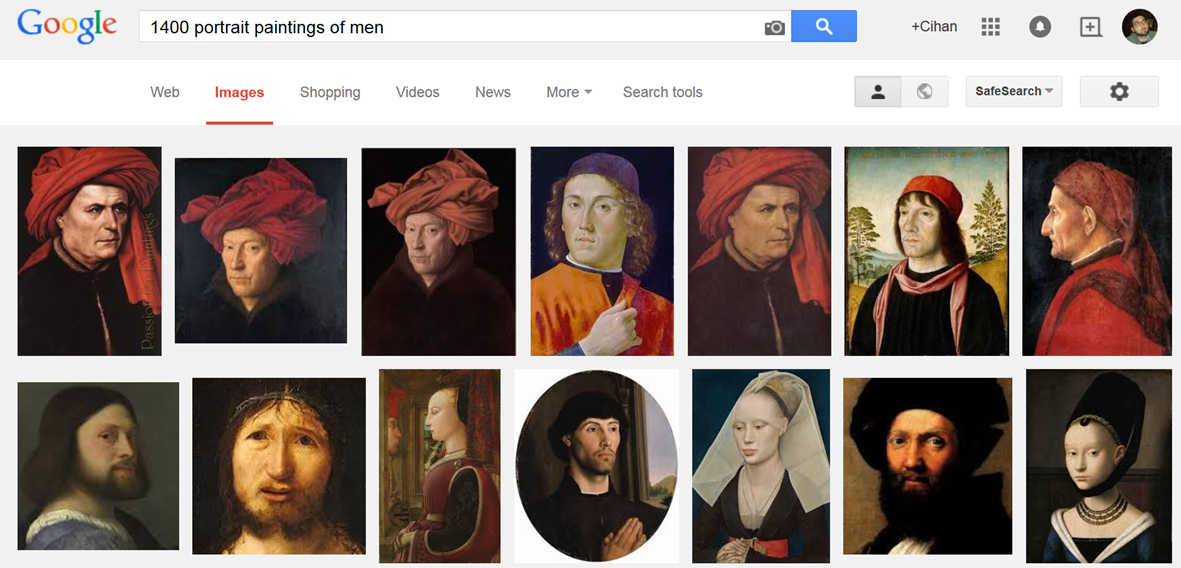
\includegraphics[width=.8\textwidth]{PaintingRecognizer-query_results}
	\caption{Google Image search results}
	\label{pr-googleres}	
\end{figure}

Viola-Jones\cite{viola} face detection is used on the downloaded images for face detection. From the face bounding box, a vector is generated pointing downwards with a distance around one face height to pointing the clothing in the portrait.

\begin{figure}
	\centering
	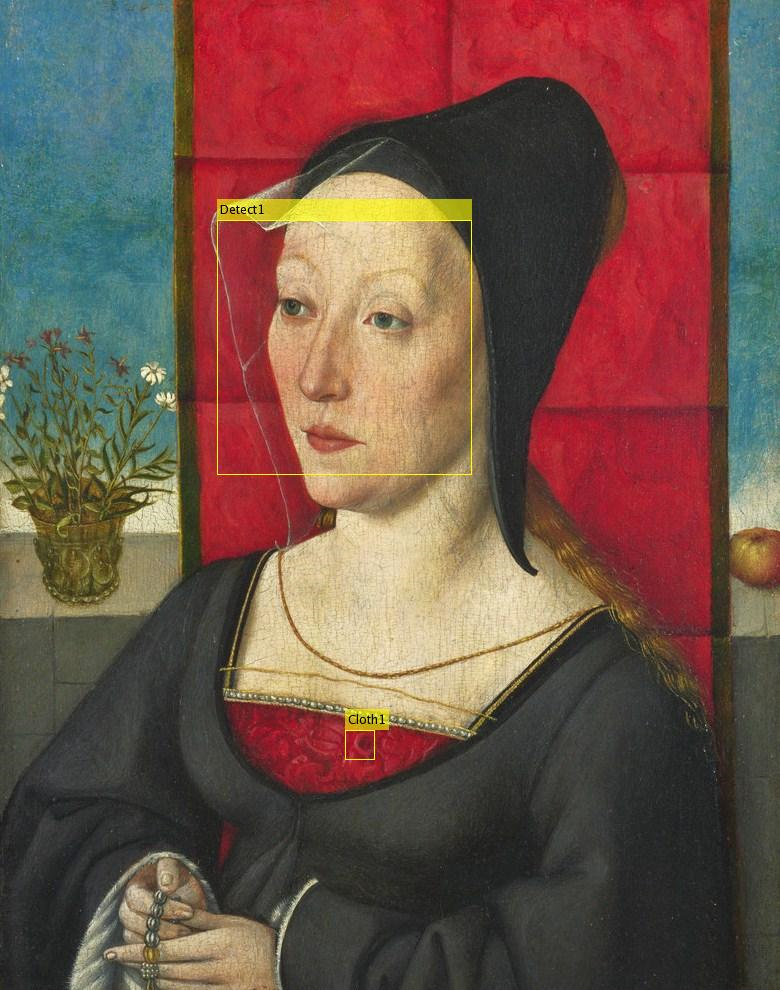
\includegraphics[width=.5\textwidth]{PaintingRecognizer-matlab_results}
	\caption{Painting Recognizer process}
	\label{pr-process}	
\end{figure}

A small rectangle around the clothing is used for color analysis. Example image given in Figure \ref{pr-process}. 

RGB intensity values are then used to compute five dominant colors per 3 years window per gender using k-means (with $k=5$). The representation of the data over time can be seen in Figure \ref{pr-result}.

\begin{figure}
	\centering
	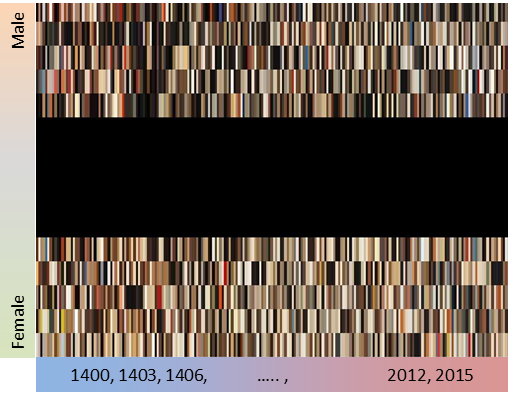
\includegraphics[width=.5\textwidth]{PaintingRecognizer-results}
	\caption{Painting Recognizer results}
	\label{pr-result}	
\end{figure}


\section{Conclusions}

\clearpage

\bibliographystyle{splncs}
\bibliography{mysubmission}
\end{document}
